\subsubsection{Rationale/Context}
A traveller might want to add a number of passengers on their ticket because of a change in plans. They can do that until one week before the departure date. If the ticket's information is updated they might have to pay an additional costs.
\subsubsection{User story}
As an employee, I want to update information of a certain ticket.
\subsubsection{Use Case}
\creator{\studentB}
\updater{\studentC}
\secondUpdater{\studentA}

\textbf{Use Case Name:} Adding extra passengers to a ticket.

\textbf{Scope:} Tickets reservation system

\textbf{Level:} User Goal

\textbf{Primary Actor:} KOENDES Employee

\textbf{Stakeholders and Interests:} 
\begin{itemize}
\item \textit{Stakeholder}: KOENDES Employee (wants fast, easy, and accurate retrieval and entry of data)
\item \textit{Stakeholder}: Traveller (Wants to be informed once the item is updated)
\end{itemize}
\textbf{Preconditions:} 
\begin{itemize}
\item Employee is authenticated
\item Employee is authorised to access this use case.
\item The ticket exists in the system.
\item The departure date is more than a week after the update request.
\end{itemize}

\textbf{Success Guarantee (Postconditions):} 
\begin{itemize}
\item State change: The information has been updated if the departure date of the ticket is one week after. Otherwise, nothing happens. 
\item Output: "Sorry the update cannot be done due to the delay in request" if the departure date is within one week; otherwise "The update has been done successfully!".
\end{itemize}

\textbf{Main Success Scenario (Basic Flow):}
\begin{enumerate}
\item The user asks the system to initiate the process of updating a ticket.
\item The system sends the user an empty search form for tickets.
\item The user enters the ticket's information provided by traveller such as reservation date or ticket's number.
\item The user sends the filled search form to the system.
\item The system sends back a ticket that matches the search query.
\item The user asks the system to update the selected ticket.
\item The system sends an update form with the actual number of passengers and possible payment methods.
\item The user fills in the number of passengers and the payment method.
\item The system calculates the new price and show it to the user.
\item The user sends the filled update form to the system.
\item The system updates the ticket.
\item The system informs the user with the final result.
\end{enumerate}
Extensions:
\begin{enumerate}
\item[8a] If the payment method can not be processed then the payment should happen before checking-in at the time of travelling.
\end{enumerate}
%\textbf{Alternate Flow:} Alternate Flow

%\textbf{Special Requirements:} Special Requirements

\textbf{Technology And Data Variations List:} 
\begin{itemize}
    \item Last name: String with alphabetical characters only
    \item Reservation date: Date of the form DD/MM/YYYY
    \item Ticket's number: Numerical string
    \end{itemize}
\textbf{Frequency of Occurrence:} 
\begin{itemize}
    \item Regularly, it really depends on the amount of passengers.
\end{itemize} 
%\textbf{Open Issues:} Open Issues

\subsubsection{SSD}
\creator{\studentB}
\updater{\studentC}
\secondUpdater{\studentA}
\\
The previous section is necessary for the creation of the SSD:
%\updater{Name \textsc{Surname}}
%\secondUpdater{Name \textsc{Surname}}
Considering the previous sub-sections we can create the following SSD model:\\\\
User $\rightarrow$ System: UpdateTicket;\hfill /* 1\\
System $\rightarrow$ User: Empty tickets search form;\hfill /* 2\\
User $\rightarrow$ User: Adding the provided information from the traveller to the search form;\hfill /* 3\\
User $\rightarrow$ System: Filled-in search form;\hfill /* 4\\
System $\rightarrow$ User: The Ticket that matches the search query;\hfill /* 5\\
User $\rightarrow$ System: UpdateTicket(Ticket);\hfill /* 6\\
System$\rightarrow$ User: An update form;\hfill /* 7\\
User $\rightarrow$ User: Adding the information to the update form;\hfill /* 8\\
System $\rightarrow$ System: Calculate the new price and show it to the user;\hfill /* 9\\
User $\rightarrow$ System: Filled-in update form;\hfill /* 10\\
System $\rightarrow$ System: Update Ticket(Number of passengers, Payment method, Price);\hfill /* 11\\
System $\rightarrow$ User: "The ticket has been updated!"\hfill /* 12\\

%\includegraphics[scale=0.9]{UC1}
\newpage
\subsubsection{Grey box SD}
\creator{\studentA}
\updater{\studentB}
\begin{figure}[H]
    \centering
    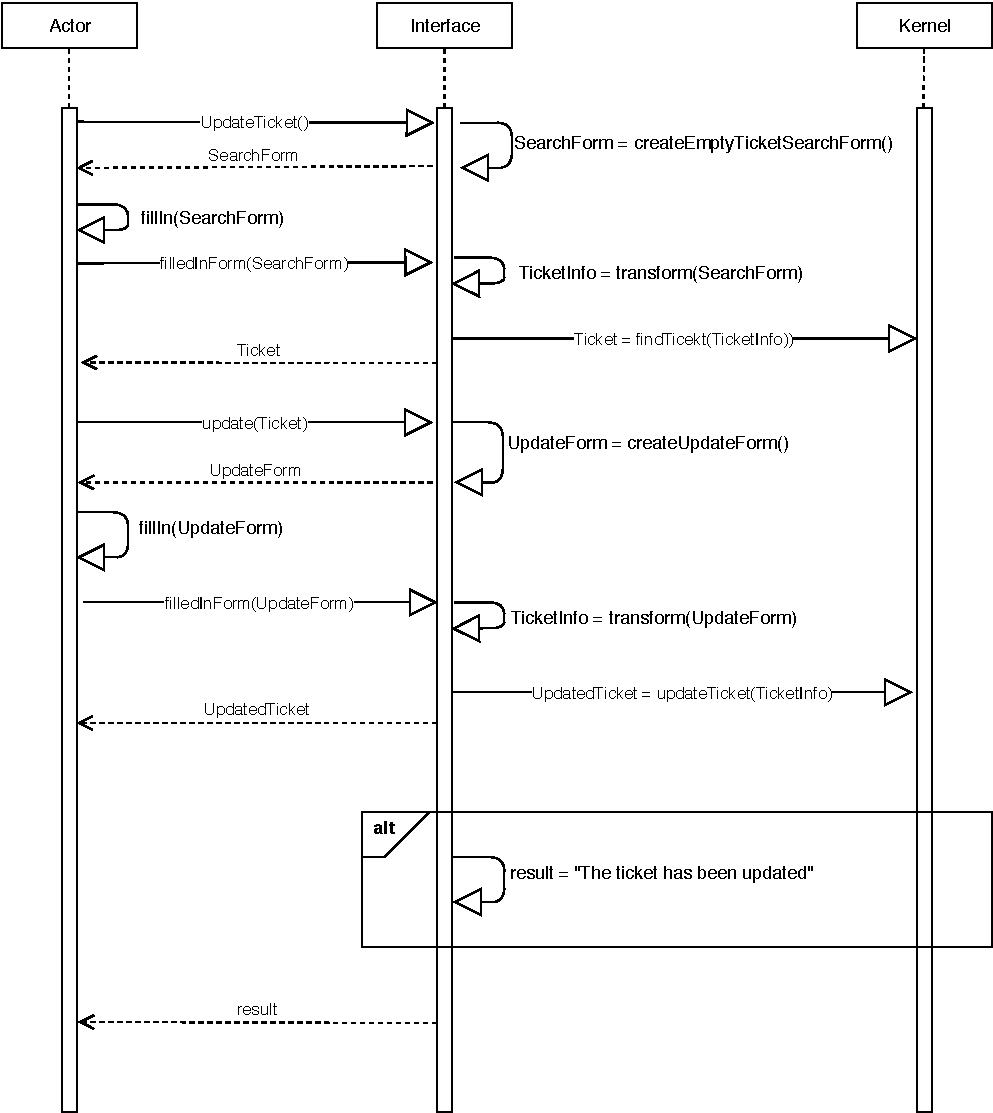
\includegraphics[scale=0.8]{Iteration_3/Files/graybox_uc2.pdf}
    \caption{6:2 Grey box}
    \label{fig:6.2 Greybox}
\end{figure}

\iffalse
\subsubsection{Whte box SD}
\creator{Name \textsc{Surname}}
\updater{Name \textsc{Surname}}

%\includegraphics[scale=0.9]{UC1wb.pdf}
\fi
\subsubsection{White box SD}
\creator{\studentA}
\updater{\studentB}
\begin{figure}[H]
    \centering
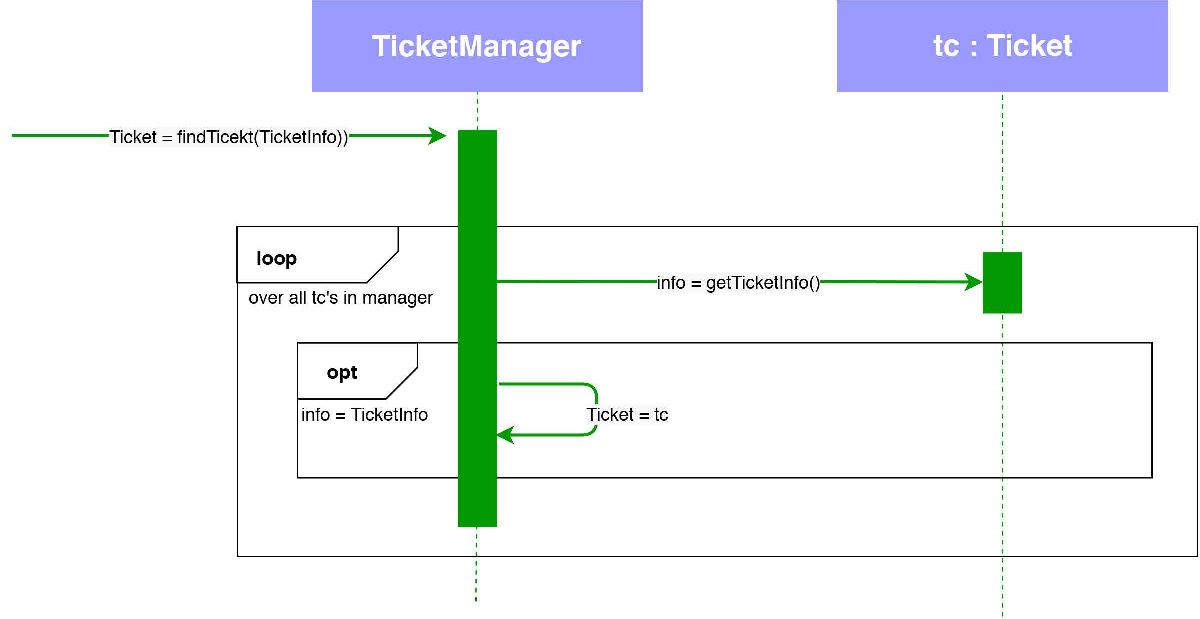
\includegraphics[scale=0.7]{Iteration_3/Files/UC2_wb1.pdf}
\end{figure}
\begin{figure}[H]
    \centering
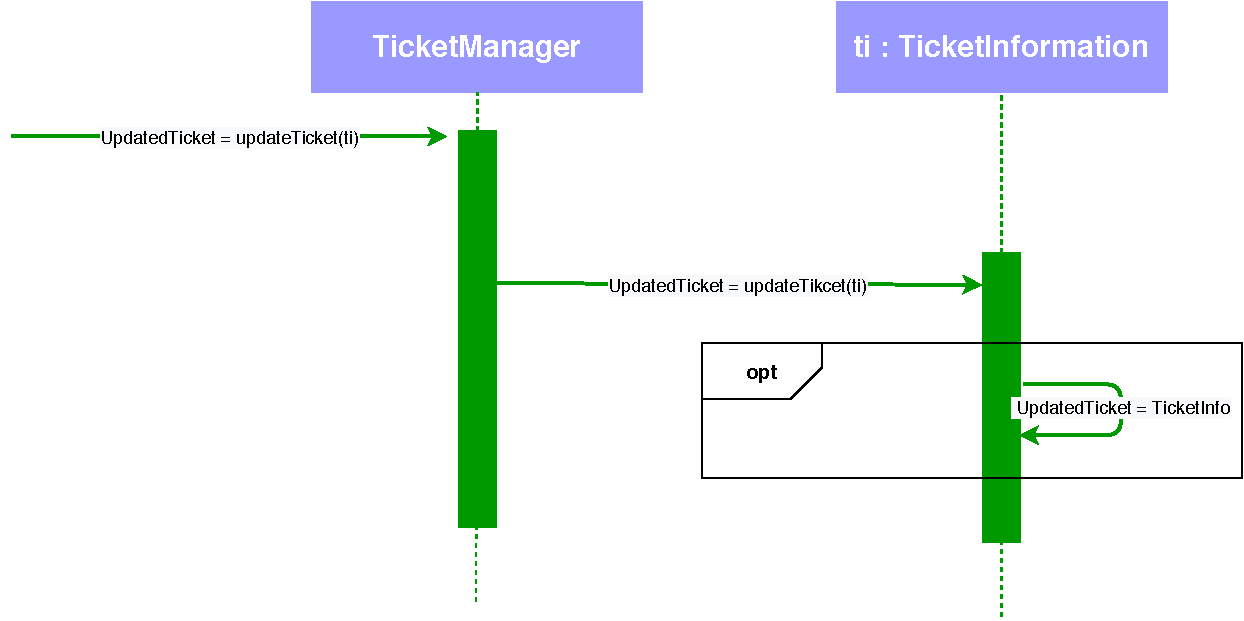
\includegraphics[scale=0.7]{Iteration_3/Files/UC2_wb3.pdf}
\end{figure}

